\documentclass[11pt,a4paper]{article}
\usepackage[utf8]{inputenc}
\usepackage[french]{babel}
\usepackage[T1]{fontenc}
\usepackage{amsmath}
\usepackage{amsfonts}
\usepackage{amssymb}
\usepackage{graphicx}
\usepackage{setspace}
\usepackage{gensymb} %Pour le degré
\usepackage{titlesec} %Pour le 3ème niveau de titres
\usepackage{fancyvrb} %Pour le Verbatim
\usepackage{alltt} %Environnement pseudo code

\newcommand{\reporttitle}{Rapport final}
\newcommand{\reportauthor}{Clément \textsc{Tamines} Jérémy \textsc{Gheysen}}
\newcommand{\reportsubject}{Projet de Structures de Données II}
\newcommand{\HRule}{\rule{\linewidth}{0.5mm}}
\renewcommand{\ttdefault}{txtt} %Pour le gras environnement pseudo-code

\setcounter{secnumdepth}{4}
\titleformat{\paragraph}
{\normalfont\normalsize\bfseries}{\theparagraph}{1em}{}
\titlespacing*{\paragraph}
{0pt}{3.25ex plus 1ex minus .2ex}{1.5ex plus .2ex}

\makeindex
\begin{document}
%TODO : Ajouter à la table des matières les paragraphes

%Page de garde
\begin{titlepage}
\begin{center}
\begin{minipage}[t]{0.48\textwidth}
  \begin{flushleft}
     
\includegraphics[width=42mm]{UMONS+txt.pdf} \\[0.5cm]
  \end{flushleft}
\end{minipage}
\begin{minipage}[t]{0.48\textwidth}
  \begin{flushright}
    
\includegraphics [width=42mm]{UMONS_FS.pdf} \\[0.5cm]
  \end{flushright}
\end{minipage} \\[1.5cm]

\vspace{1.5cm}
\textsc{\Large \reportsubject}\\[0.5cm]
\HRule \\[0.4cm]
{\huge \bfseries \reporttitle}\\[0.4cm]
\HRule \\[1.5cm]

\begin{minipage}[t]{0.3\textwidth}
  \begin{flushleft} \large
    \emph{Auteurs :}\\
    \reportauthor
  \end{flushleft}
\end{minipage}
\begin{minipage}[t]{0.6\textwidth}
  \begin{flushright} \large
    \emph{Professeur :} \\
    V. \textsc{Bruyère} \\
     \emph{Assistant :} \\
    G. \textsc{Devillez}
  \end{flushright}
\end{minipage}
\vfill
{\large 15 avril 2016}

\end{center}
\end{titlepage}

\tableofcontents
\newpage

\section*{Introduction}
\addcontentsline{toc}{section}{Introduction}
Ce projet consiste en l'implémentation d'un outil permettant la représentation, en 2 dimensions, de scènes formées d'un ensemble de segments colorés placés dans un repère orthonormé. Cette représentation comprend deux paramètres ajustables à souhait : un point de vue pouvant se situer à divers endroits dans le repère, et un certain angle de vision $\alpha$ tel que $0 \degree <\alpha<180 \degree$.\\

Pour réaliser cet affichage, nous utiliserons comme décrit dans l'énoncé l'algorithme du peintre. Ce dernier se basant sur des arbres de type BSP (\emph{Binary Spaces Partition}), il nous faut d'abord, à partir d'une liste de segments définis par leurs sommets et leur couleur, construire ces arbres. Leur création peut se faire de différentes manières, nous utiliserons ici 3 techniques : la technique classique "inordre", sa variante "random" et le principe des "free-splits". \\

Ce rapport a pour but de décrire et expliquer les différentes techniques et algorithmes utilisés lors de la construction des arbres BSP et de la visualitation de ces derniers à l'aide de l'algorithme du peintre. Nous analyserons également la complexité et la performance de tels algorithmes.

\newpage

\section{Arbres BSP}
\subsection{Principe}
Un arbre BSP (\emph{Binary Space Partition}), est un arbre binaire permettant de stocker de manière efficace un ensemble d'objets (dans notre cas de segments) situés dans un plan. Rappelons tout de même qu'un arbre binaire est un arbre tel que tout noeud possède au plus deux fils. \\

Le type d'arbre étudié ici consiste donc en une séparation binaire de l'espace, s'effectuant de manière récursive. C'est à dire que chaque noeud, possédant un ensemble de segments restants dans le plan, définit une nouvelle séparation binaire de ce dernier, cela sur base d'une droite (choisie selon une technique définie au préalable, contenant un, ou plusieurs segments s'ils ont la même équation), et sépare ainsi le plan en deux sous-espaces contenant chacun une partie des segments restants. Cette méthode est alors appelée récursivement sur chacun des deux sous-espaces nouvellement créés (les deux fils) jusqu'au moment où tous les segments présents dans le plan sont contenus dans les noeuds de l'arbre. L'utilisation de la droite pour définir les nouveaux plans peut néanmoins couper des segments restants en deux, le segment original est alors supprimé et les deux nouveaux segments sont alors placés dans le fils leur correspondant en fonction de leur position. Remarquons qu'avec la manière avec laquelle nous définissons chaque nouveau noeud, les feuilles sont également des noeuds définissant deux nouveaux plans, mais ces derniers ne contiendront alors aucun segment (appel récursif alors impossible). \\

La taille d'un arbre BSP est calculée en fonction du nombre total des noeuds le constituant. Moins il y aura eu de fragmentation lors de la création de l'arbre, moins ce dernier sera grand et inversément. Il est donc intéressant de limiter cette fragmentation. \\

Il existe bien évidemment diverses méthodes afin de construire de tels arbres de manière plus ou moins optimisée (en taille et/ou en temps), nous verrons ci-dessous trois de ces méthodes. 

\subsection{Éléments indispensables à la construction}

\subsubsection{Segment}
La classe Segment, permet, comme son nom l'indique, de représenter un segment dans le plan orthonormé, son constructeur prend en paramètres ses deux extrémités $(x1,y1)$, $(x2,y2)$ et sa couleur. Un segment possède également trois autres paramètres (\emph{intersected, isFreeSplit, intersection}), nécessaires à l'implémentation de l'heuristique des free-splits. Nous nous attarderons sur ces éléments plus tard. \\
Au niveau des méthodes, passons en revue les plus importantes, étant des outils très importants pour la suite des calculs :
\begin{itemize}
\item \emph{computeLine} : Calcule la droite générée à partir du segment en question;
\item \emph{getSide} : Cette méthode remplace les coordonnées $x$ et $y$ données en paramètres dans la droite également donnée en paramètre et retourne le résultat (donc 0 si le point est sur la droite);
\item \emph{computePosition} : Retourne la position relative du segment par rapport à la droite donnée en paramètre. Remarquons que pour cette méthode certaines conventions ont été prises. En effet, s'il y a intersection, cette dernière est retournée. Sinon, si le segment est à gauche de la droite, NaN est retourné, s'il est à droite, c'est Infinity qui est renvoyé. Notons également que si nous nous trouvons dans le cas où il y a intersection au niveau d'un sommet du segment, par facilité d'implémentation nous retournons NaN ou Infinity en fonction de sa position et non le point d'intersection. Car en effet, nous aurions sinon création d'un segment qui est en réalité un point lors de la création de l'arbre BSP (ce qui aurait consisté en une segmentation incorrecte).
\end{itemize}

\subsubsection{BSPNode} 
Cette classe est utile pour le stockage des arbres BSP. Sa conception est très proche des structures utilisées de manière standard pour la représentation de simples arbre binaire. Des adaptations ont uniquement été faites pour stocker dans chaque noeud le ou les segment(s) présent(s) dans la droite le caractérisant, et les segments présents dans l'hyperplan défini par le père (tous les segments s'il s'agit de la racine). 

\subsection{Construction}
\subsubsection{Heuristique "in-order"}

\paragraph{Méthode}

Cette heuristique, facile à réaliser, est très intuitive et met simplement en pratique le principe des arbres BSP. Étudions son fonctionnement à l'aide de l'exemple représenté à la Figure \ref{scene_inordre} : 

\begin{figure}[!h]
\centering
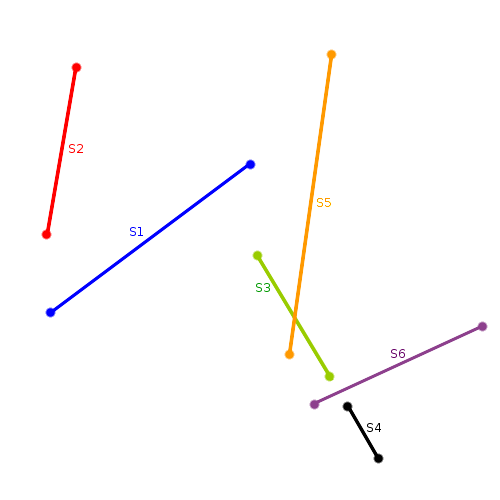
\includegraphics[scale=0.6]{bsp_ex_1.png}
\caption{Scène 2D}
\label{scene_inordre}
\end{figure}

Nous pouvons remarquer que cette scène contient 6 segments distincts, dont deux (les segments S3 et S4) se situant sur une même droite. Nous avons également des segments qui s'intersectent, ce qui va inexorablement mener à la création de nouveaux segments. Nous allons maintenant appliquer et expliquer le fonctionnement de l'heuristique "inordre", celui-ci étant représenté dans le plan à la Figure \ref{bsp_inordre} et l'arbre BSP correspondant est construit à la Figure \ref{bsp_tree}. \\

Cette heuristique travaille avec la liste des segments telle qu'elle a été fournie par l'utilisateur, c'est à dire que la création de l'arbre se fait dans l'ordre par lequel les segments ont été définis. \\

Nous commençons donc par une division du plan à l'aide de S1, et nous remarquons d'ores et déjà que S5 est alors coupé en deux segments S5A et S5B, en effet S5 intersecte la droite issue du prolongement de S1. Nous obtenons donc maintenant deux sous-ensembles de segments : 
$$S1^+ = \{S2, S5A\}$$
$$S1^- = \{S3,S4,S5B,S6\}$$
Récursivement, l'algorithme va être appelé sur $S1^+$ et $S1^-$. Et c'est le premier segment de la liste qui sera utilisé comme nouvelle droite définissant les nouveaux plans. 
\begin{itemize}
\item Pour $S1^+$ on a donc ainsi $S2$ comme segment de base pour la nouvelle droite. Il ne restera ainsi plus que $S5A$ comme feuille. 
\item Pour $S1^-$ on a $S3$ comme origine de la nouvelle droite et on remarque que $S4$ est également inclu à la droite, donc ces deux segments font alors partie du même noeud. Nous avons également que $S3$ intersecte $S5B$ et $S6$ ce qui engendre la création des segments : $S5C$, $S6A$, $S6B$, la suppression du segment $S6$ et la modification de $S5B$ (qui se traduira néanmoins techniquement par la suppression et la création d'un segment avec les coordonnées mises à jour). 
\end{itemize}

\begin{figure}[!h]
\centering
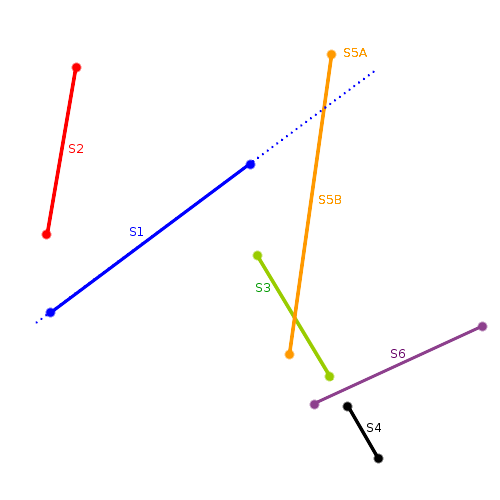
\includegraphics[scale=0.6]{bsp_ex_2.png}
\caption{Application de l'heuristique}
\label{bsp_inordre}
\end{figure}

\begin{figure}[!h]
\centering
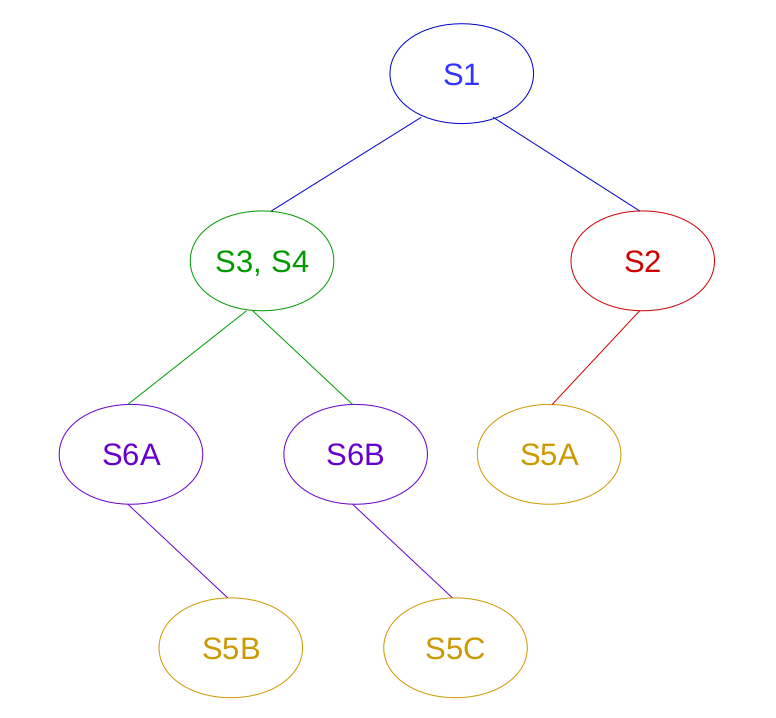
\includegraphics[scale=0.35]{bsp_ex_3.png}
\caption{Arbre BSP}
\label{bsp_tree}
\end{figure}

\paragraph{Implémentation}

Afin d'implémenter cette heuristique, nous utilisons principalement les 2 algorithmes suivants :
\begin{itemize}
\item createTree : permet de lancer la création de l'arbre;
\item createRoot : assure la construction récursive de l'arbre à partir d'un noeud;
\end{itemize}

Notons que nous utilisons les conventions suivantes :
\begin{itemize}
\item La création d'un noeud nécessite 4 paramètres : fils droit, fils gauche, la liste de segments de l'hyperplan et la droite effectuant la définition des deux nouveaux hyperplans (communément appelée "splitting line").
\item Un noeud possède 5 attributs : rightSon, leftSon, segmentsInHyperplane (liste des segments dans l'hyperplan défini par le droite de séparation du père), segmentsInLine (segments dans la ligne de séparation), line (tableau de trois doubles étant les facteurs a, b et c de l'équation de sa droite de séparation).
\item Un noeud possède entre autres les deux méthodes setLeftSon et setRightSon permettant d'ajouter respectivement un fils gauche et/ou un fils droit au noeud. 
\end{itemize}

\begin{alltt}
\textbf{createTree}
Entrée : segList, liste de segments d'origine pour la création 
de l'arbre BSP
Sortie : racine de l'arbre BSP généré

1: \(line \leftarrow segList[0]\)
2: enlever \(segList[0]\) de \(segList\)
3: \(racine\) \(\leftarrow\) nouveau noeud (\(vide\), \(vide\), \(segList\), \(line\))
4: createRoot(\(racine\))
5: retourner \(racine\)
\end{alltt}

\begin{alltt}
\textbf{createRoot}
Entrée : noeud, étant un noeud incomplet de l'arbre BSP ne
disposant que de sa ligne de séparation et sa liste de
segments contenus dans son hyperplan.
Sortie : /
Effet : ajoute les fils au noeud s'il en a et dans ce cas 
appelle l'algorithme récursivement sur ces derniers en 
choisissant une nouvelle droite de séparation et en 
donnant les nouvelles listes de segments adaptées.

 1: si \(noeud\) non vide alors
 2:   pour chaque segment \(s\) dans \(noeud.segmentsInHyperplane\) faire
 3:     si \(s \in noeud.line\) alors
 4:       ajouter \(s\) à \(segmentsInLine\)
 5:       enlever \(s\) de \(segmentsInHyperplane\)
 6:       
 7:   créer les listes \(leftNodeSegments\) et \(rightNodeSegments\)
 8:   
 9:   pour chaque segment \(s\) dans \(noeud.segmentsInHyperplane\) faire
10:     si \(s\) est à droite de \(noeud.line\) alors
11:       ajouter \(s\) à \(rightNodeSegments\)
12:
13:     sinon si \(s\) est à gauche de \(noeud.line\) alors
14:       ajouter \(s\) à \(leftNodeSegments\)
15:
16:     sinon on est dans le cas où \(s\) intersecte \(noeud.line\) alors
17:       créer deux nouveaux segments \(s1\) et \(s2\)
18:       si \(s1\) est à droite de \(noeud.line\) alors
19:         ajouter \(s1\) à \(rightNodeSegments\)
20:         ajouter \(s2\) à \(leftNodeSegments\)
21:
22:       sinon
23:         ajouter \(s1\) à \(leftNodeSegments\)
24:         ajouter \(s2\) à \(rightNodeSegments\)
25:         
26:   si \(leftNodeSegments\) et \(rightNodeSegments\) sont non-vides alors
27:     \(line \leftarrow rightNodeSegments[0]\)
28:     enlever \(rightNodeSegments[0]\) de \(rightNodeSegments\)
29:     \(rightNode \leftarrow\) nouveau noeud (\(vide\), \(vide\), \(rightNodeSegments\), \(line\))
30:     setRightSon(\(rightNode\))
31:     \(line \leftarrow leftNodeSegments[0]\)
32:     enlever \(leftNodeSegments[0]\) de \(leftNodeSegments\)
33:     \(leftNode \leftarrow\) nouveau noeud (\(vide\), \(vide\), \(leftNodeSegments\), \(line\))
34:     setLeftSon(\(leftNode\));
35:     
36:   sinon si \(leftNodeSegments\) vide et \(rightNodeSegments\) non-vide alors
37:     \(line \leftarrow rightNodeSegments[0]\)
38:     enlever \(rightNodeSegments[0]\) de \(rightNodeSegments\)
39:     \(rightNode \leftarrow \) nouveau noeud (\(vide\), \(vide\), \(rightNodeSegments\), \(line\))
40:     setRightSon(\(rightNode\))
41:    
42:   sinon si \(leftNodeSegments\) non-vide et \(rightNodeSegments\) vide alors
43:     \(line \leftarrow leftNodeSegments[0]\)
44:     enlever \(leftNodeSegments[0]\) de \(leftNodeSegments\)
45:     \(leftNode \leftarrow \) nouveau noeud (\(vide\), \(vide\), \(leftNodeSegments\), \(line\))
46:     setLeftSon(\(leftNode\))
47:     
48:   createRoot(\(leftNode)\))
49:   createRoot(\(rightNode\))
\end{alltt}

Pour effectuer la création d'un arbre BSP avec l'heuristique "inordre" nous appelons simplement createTree avec la liste des segments devant former l'arbre. Cet algortihme va alors se charger d'initialiser le premier noeud en utilisant le premier segment de la liste comme droite de séparation. Ensuite l'algorithme createRoot est appelé avec ce premier noeud, c'est cet algorithme qui se charge ensuite de la construction récursive de l'arbre. \\

Tout d'abord, l'instruction 1 permet de ne faire fonctionner l'algorithme que s'il a du sens, c'est à dire que le noeud sur lequel il est appelé est non nul. Nous pouvons ensuite effectuer une analyse en deux parties : 

La première partie, constituée des instructions 2 à 25, consiste en la création de deux nouveaux hyperplans en fonction de la "splitting line" du noeud. On regarde d'abord si des segments de l'hyperplan du noeud sont contenus dans cette droite et, s'ils existent, on les ajoute à la liste des segments contenus dans la droite. Ensuite, avec les segments restants, on va regarder s'ils se situent à gauche ou à droite de la "splitting line" pour ensuite pouvoir les répartir correctement (dans le cas où il y a intersection, on crée deux nouveaux segments et on les ajoute au bon nouvel hyperplan en fonction de leur position). 

La seconde partie permet la création de la structure d'arbre en tant que tel, constituée des instructions 26 à 49 elle va simplement attribuer au noeud un fils gauche et un fils droit. Si de tels fils existent (car on peut être dans le cas d'un noeud), leur hyperplan correspondant, calculé dans la première partie, leur est attribué et une nouvelle droite de séparation (générée à partir du premier segment de l'hyperplan) leur est donnée. Ensuite l'algorithme est appelé récursivement sur ces deux fils. 

\paragraph{Complexité}

\subsubsection{Heuristique "random"}

\paragraph{Méthode}

Cette heuristique utilise la même méthode que l'heuristique "inordre" pour la création de l'arbre BSP, à la seule différence près que la liste des segments est mélangée avant de commencer la construction. La différence d'un point de vue algorithmique avec l'heuristique précédente étant nulle, nous ne attardons donc pas sur ce point. 

\paragraph{Implémentation}

L'implémentation de cette heuristique est identique à la précédente à l'exception d'une ligne effectuant le mélange de la liste des segments avant utilisation. On va donc ici mélanger la liste des segments, puis appeler l'algorithme précédent :

\begin{alltt}
\textbf{createTree}
Entrée : segList, liste de segments d'origine pour la création 
de l'arbre BSP
Sortie : racine de l'arbre BSP généré

1: \(inorder \leftarrow\) nouveau InOrderHeuristic()
2: mélanger \(segList\)
3: retourner inorder.createTree(\(segList\))
\end{alltt}

\paragraph{Complexité}

N'ayant effectué qu'un mélange de liste en \emph{O(n)} en dehors de toute boucle ou appel récursif, cela n'aucun impact au niveau de la complexité asymptotique. 

\subsubsection{Heuristique "free-splits"}

\paragraph{Méthode}

Afin d'expliquer au mieux cette heuristique, nous utiliserons également un exemple, représenté à la Figure \ref{scene_splits}. \\

Cette heuristique se veut plus réfléchie que la simple utilisation, dans un ordre aléatoire ou non, des segments pour la définition de nouveaux plans. Nous allons donc étudier ici le cas particulier des "free-splits", ce dernier n'apparaissant que dans des circonstances bien précises, recréées ici dans l'exemple. Notons que cette heuristique se base sur une liste de segments ordonnés de manière aléatoire, néanmoins, pour les besoins de l'exemple nous supposerons que l'algorithme traite les segments dans l'ordre où ceux-ci ont été définis. En effet, si nous traitons les segments dans un ordre aléatoire, il se pourrait que nous soyons en présence d'une situation ne disposant pas de "free-split".

\begin{figure}[!h]
\centering
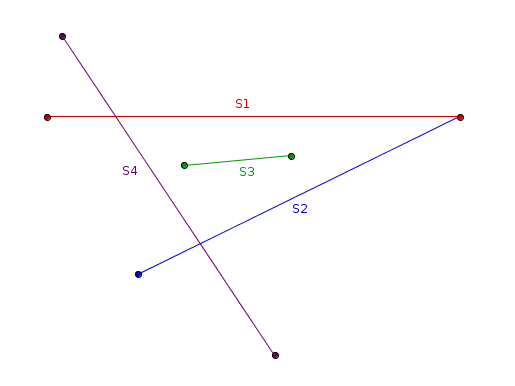
\includegraphics[scale=0.5]{free_splits_2.png}
\caption{Scène 2D}
\label{scene_splits}
\end{figure}

Exécutons pas à pas l'algorithme et définissons à l'aide de l'exemple la notion de "free-split". \\

Nous pouvons observer que cette scène est composée de 4 segments. Imaginons que nous avons déjà construit une partie de l'arbre BSP avec S1 et S2, nous remarquons alors que ces deux segments coupent S4, ce qui divise S4 en trois nouveaux segments (nommés S4A, S4B et S4C dans la Figure \ref{heuristic_splits}). A cette étape nous avons déjà la partie gauche de l'arbre construite avec S4A en tant que feuille (voir Figure \ref{split_bsp}). Il reste alors à construire le côté droit à partir de S2. S4C étant tout seul de son côté, le choix se porte alors entre S3 et S4B comme base pour une nouvelle droite. Or étant donné que S4B est déjà intersecté par deux droites, l'utiliser comme nouvelle droite ne causera pas de nouvelle fragmentation lors de la création du noeud ! C'est ce que l'on appelle la notion de "free-splits", c'est à dire utiliser des segments déjà intersectés par deux droites existantes pour définir de nouveaux plans, car ceux-ci, par conséquent ne fragmenteront plus aucun segment. Ce qui donc est avantageux au niveau de la quantité de segments qui est alors censée être réduite.\\

Notons que lorsqu'aucun "free-split" n'est présent, c'est l'algorithme classique "random" de création d'arbre BSP qui est d'application. 

\begin{figure}[!h]
\centering
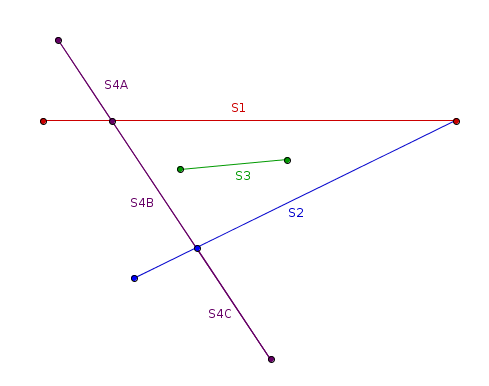
\includegraphics[scale=0.5]{free_splits_1.png}
\caption{Application de l'heuristique}
\label{heuristic_splits}
\end{figure}


\begin{figure}[!h]
\centering
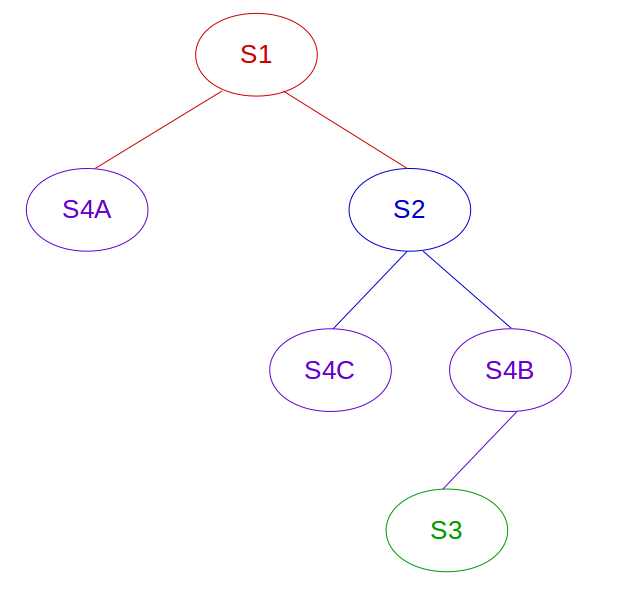
\includegraphics[scale=0.4]{free_splits_3.png}
\caption{Arbre BSP}
\label{split_bsp}
\end{figure}

\paragraph{Implémentation}

L'implémentation de l'heuristique des "free-splits" paraît à première vue fort semblable par rapport à celle "inorder", ce qui est normal étant donné qu'elles possèdent le même squelette, "free-splits" n'apportant que quelques améliorations se basant sur des conditions supplémentaires. Nous allons donc ici présenter un pseudo-code très semblable au précédent, c'est pourquoi les numéros de lignes présentant un changement seront mises en gras.\\

Pour les besoins de l'heuristique nous introduisons les attributs suivants aux objets de type segment : un booléen isIntersected indiquand si le segment a déjà été intersecté ou non, un tableau de deux nombres nommé intersection contenant cette intersection si elle existe et un booléen isFreeSplit indiquant si le segment est un "free-split". Notons également les deux abréviations suivantes : a et b pour désigner les deux extrémités du segment.\\

Notons bien qu'afin de comprendre sans ambiguïté les lignes 20,25,27 et 30, nous admettons que lorsque nous réalisons une coupure au niveau d'un segment par une droite, celle-ci se fait au niveau de l'extrémité b pour les nouveaux segments. 

\begin{alltt}
\textbf{createTree}
Entrée : segList, liste de segments d'origine pour la création 
de l'arbre BSP
Sortie : racine de l'arbre BSP généré

\textbf{1:} mélanger \(segList\)
2: \(line \leftarrow segList[0]\)
3: enlever \(segList[0]\) de \(segList\)
4: \(racine\) \(\leftarrow\) nouveau noeud (\(vide\), \(vide\), \(segList\), \(line\))
5: createRoot(\(racine\))
6: retourner \(racine\)
\end{alltt} 

\begin{alltt}
\textbf{createRoot}
Entrée : noeud, étant un noeud incomplet de l'arbre BSP ne
disposant que de sa ligne de séparation et sa liste de
segments contenus dans son hyperplan.
Sortie : /
Effet : ajoute les fils au noeud s'il en a et dans ce cas 
appelle l'algorithme récursivement sur ces derniers en 
choisissant une nouvelle droite de séparation et en 
donnant les nouvelles listes de segments adaptées.

 1: si \(noeud\) non vide alors
 2:   pour chaque segment \(s\) dans \(noeud.segmentsInHyperplane\) faire
 3:     si \(s \in noeud.line\) alors
 4:       ajouter \(s\) à \(segmentsInLine\)
 5:       enlever \(s\) de \(segmentsInHyperplane\)
 6:       
 7:   créer les listes \(leftNodeSegments\) et \(rightNodeSegments\)
 8:   
 9:   pour chaque segment \(s\) dans \(noeud.segmentsInHyperplane\) faire
10:     si \(s\) est à droite de \(noeud.line\) alors
11:       ajouter \(s\) à \(rightNodeSegments\)
12:
13:     sinon si \(s\) est à gauche de \(noeud.line\) alors
14:       ajouter \(s\) à \(leftNodeSegments\)
15:
16:     sinon on est dans le cas où \(s\) intersecte \(noeud.line\) alors
17:       créer deux nouveaux segments \(s1\) et \(s2\)
18:
\textbf{20:}		      si \(s\) est intersecté et intersection \(=s1.a\) alors
\textbf{21:}		        \(s1\) devient un free-split
\textbf{22:}		    
\textbf{23:}		      sinon
\textbf{24:}		        \(s1\) devient intersecté
\textbf{25:}		        \(s1.intersection\) = \(s1.b\)
\textbf{26:}		    
\textbf{27:}		      si \(s\) est intersecté et intersection \(=s2.a\) alors
\textbf{28:}		        \(s2\) devient un free-split
\textbf{29:}		    
\textbf{30:}		      sinon
\textbf{31:}		        \(s2\) devient intersecté
\textbf{32:}		        \(s2.intersection\) = \(s2.b\)
33:		
34:       si \(s1\) est à droite de \(noeud.line\) alors
35:         ajouter \(s1\) à \(rightNodeSegments\)
36:         ajouter \(s2\) à \(leftNodeSegments\)
37:
38:       sinon
39:         ajouter \(s1\) à \(leftNodeSegments\)
40:         ajouter \(s2\) à \(rightNodeSegments\)
41:   
\textbf{42:}	  \(fsLeft = faux\)
\textbf{43:}	  \(fsRight = faux\)
\textbf{44:}      
\textbf{45:}   si taille de \(leftNodeSegments < 1\)
\textbf{46:}     pour chaque segment \(s\) dans \(leftNodeSegments\) faire
\textbf{47:}       si \(s\) est free-split
\textbf{48:}         \(fsLeft = true\)
\textbf{49:}         enlever \(s\) de \(leftNodeSegments\)
\textbf{50:}         \(leftNode \leftarrow \) nouveau noeud (\(vide\), \(vide\), \(leftNodeSegments\), \(s\))
\textbf{51:}         setLeftSon(\(leftNode\))
\textbf{52:}            
\textbf{53:}    si taille de \(rightNodeSegments < 1\)
\textbf{54:}      pour chaque segment \(s\) dans \(rightNodeSegments\) faire
\textbf{55:}        si \(s\) est free-split
\textbf{56:}          \(right = true\)
\textbf{57:}          enlever \(s\) de \(rightNodeSegments\)
\textbf{58:}          \(rightNode \leftarrow \) nouveau noeud (\(vide\), \(vide\), \(rightNodeSegments\), \(s\))
\textbf{59:}          setrightSon(\(rightNode\))
60:
61:   si \(leftNodeSegments\) et \(rightNodeSegments\) sont non-vides alors
\textbf{62:}	    si \(fsRight\) est faux
63:       \(line \leftarrow rightNodeSegments[0]\)
64:       enlever \(rightNodeSegments[0]\) de \(rightNodeSegments\)
65:       \(rightNode \leftarrow\) nouveau noeud (\(vide\), \(vide\), \(rightNodeSegments\), \(line\))
66:       setRightSon(\(rightNode\))
67
\textbf{68:}	    si \(fsLeft\) est faux
69:       \(line \leftarrow leftNodeSegments[0]\)
70:       enlever \(leftNodeSegments[0]\) de \(leftNodeSegments\)
71:       \(leftNode \leftarrow\) nouveau noeud (\(vide\), \(vide\), \(leftNodeSegments\), \(line\))
72:       setLeftSon(\(leftNode\));
73:     
\textbf{74:}   sinon si \(leftNodeSegments\) vide et \(rightNodeSegments\) non-vide et
\textbf{75:}   \(fsLeft\) est faux alors
76:     \(line \leftarrow rightNodeSegments[0]\)
77:     enlever \(rightNodeSegments[0]\) de \(rightNodeSegments\)
78:     \(rightNode \leftarrow \) nouveau noeud (\(vide\), \(vide\), \(rightNodeSegments\), \(line\))
79:     setRightSon(\(rightNode\))
80:    
\textbf{81:}   sinon si \(leftNodeSegments\) non-vide et \(rightNodeSegments\) vide 
\textbf{82:}   et \(fsRight\) est faux alors
83:     \(line \leftarrow leftNodeSegments[0]\)
84:     enlever \(leftNodeSegments[0]\) de \(leftNodeSegments\)
85:     \(leftNode \leftarrow \) nouveau noeud (\(vide\), \(vide\), \(leftNodeSegments\), \(line\))
86:     setLeftSon(\(leftNode\))
87:     
88:   createRoot(\(leftNode)\))
89:   createRoot(\(rightNode\))
\end{alltt}

Au niveau du code présent aux lignes 20-32, il s'agit de la recherche de free-splits. En effet ceux-ci peuvent se créer lorsqu'il y a une coupure d'un segment par une droite. Ce dernier, si déjà intersecté précédemment, présente alors un free-split sur un de ses sous-segments récemment créés. C'est ce que nous réalisons aux lignes 20-21 et 27-28, en vérifiant bien si nous nous trouvons sur le bon sous-segment. Par contre si le segment original n'a pas encore été intersecté, nous marquons les deux sous-segments comme intersectés et conservons dans une variable le point d'intersection. \\

Pour les instructions 42-59, il s'agit simplement d'une vérification permettant de savoir si des free-splits sont présent dans la liste des segments pour le fils gauche et le fils droit. Si c'est le cas, le noeud est créé avec le segment résultant du free-split comme base pour une nouvelle droite de séparation, un booléen est mis à vrai et il n'y aura donc pas de choix aléatoire comme dans l'heuristique précédente. Et cela grâce aux conditions ajoutée en 62,68,74-75 et 81-82. Si aucun free-split n'est trouvé, le premier segment de l'hyperplan en question est choisi comme nouvelle "splitting-line", comme dans l'heuristique précédente. 

\paragraph{Complexité}

\subsection{Tests \& Résultats}

Dans cette section nous allons analyser les performances des différentes heurisitiques pour la création des arbres BSP. \\

\section{Algorithme du peintre}

\subsection{Détails sur l'algorithme}

\subsection{Implémentation}

\subsection{Tests \& Résultats}

\section{Interface graphique}

%TODO : Expliquer les subtilités de l'utilisation ? 

\section*{Conclusion}
\addcontentsline{toc}{section}{Conclusion}
\end{document}